%
% Charset: utf8
% File type: Plain LATEX
% Content: This chapter describes the supported boot methods of the Mini2440.
%
% Copyright Jürgen Beisert <jbe@pengutronix.de>, 2011
%
% This work is licensed under the Creative Commons Attribution 3.0 Unported License.
% To view a copy of this license, visit:
%           http://creativecommons.org/licenses/by/3.0/
%
% Refer the file CREDITS for all people working on this document.
%
% This file content will be part of the "OSELAS.BSP-Pengutronix-Mini2440-Quickstart.pdf"
%
% Note: This document uses some externaly defined LATEX commands. If you try to
% run LATEX only on this file it will fail due to the absense of these commands
% All these commands are starting with 'ptxdist'.
%

\chapter{How to Boot the Mini2440}	\label{sec:bootingmini2440}

Various methods are exist to bring up the Mini2440. The main difference is if
the Mini2440 can boot in a standalone manner or if it depends on some services
from another host via network.

To start the Mini2440 in a standalone manner it provides some local memory types
to store the relevant software parts.

\begin{itemize}
\item \texttt{NOR type flash memory} can be used to bring up the Mini2440. In
	this BSP NOR is used for the initial bootload of Barebox and as a
	fall-back or rescue bootloader. This allows the user to easily restore
	a "bricked" Mini2440.
\item \texttt{NAND type flash memory} provides enough memory space to hold all
	run-time relevant software parts. This board support package supports
	this memory type as one way to start the Mini2440 standalone.
\item \texttt{SD/MMC card memory} is a nice and easy way to deploy the run-time
	relevant software parts at the development host and simply booting
	the Mini2440 with it.
\end{itemize}

Note: All the mentioned boot methods below require Barebox as their bootloader.
The easiest way to get Barebox into the Mini2440 is via its internal NAND. So,
at least Barebox and its persistent environment has to be stored into the NAND
flash memory. The other parts (kernel and root filesystem) can be loaded from
all other supported media.

\section{NOR Type Flash Memory}

As the NOR type flash memory is not supported in this board support package,
we skip its explanation here.

\section{NAND Type Flash Memory}				\label{sec:nandflashmem}

This is the most common method to boot the Mini2440. It does not depend on
any external media or network connection. And it is also a fast method to
boot it.

To use the NAND flash as the boot media, this board support package creates
two files when running the last \texttt{ptxdist images} step:

\begin{itemize}
\item \texttt{\ptxdistPlatformDir images/linuximage} is the Linux kernel
	and must be stored in the corresponding NAND partition
\item \texttt{\ptxdistPlatformDir images/root.jffs2} contains the root filesystem
	and must be stored 'as is' in the corresponding NAND partition
\end{itemize}

\centerline{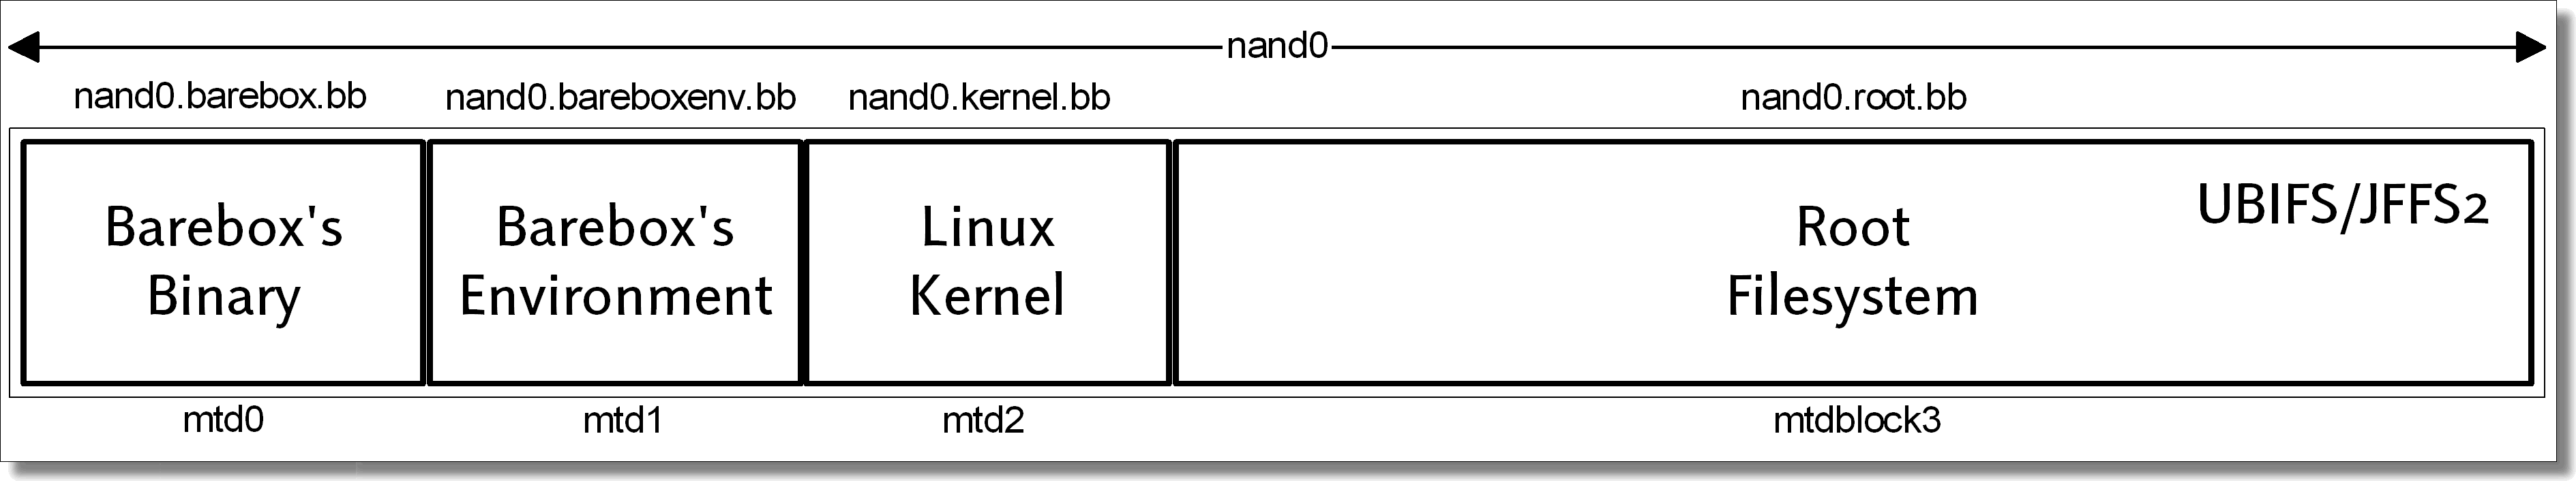
\includegraphics{OSELAS.BSP-Pengutronix-Mini2440/documentation/plain_sources/nand_partition.png}}

At our host's side:

\begin{ptxshell}[escapechar=|]{^}
|\$| cp |\ptxdistPlatformDir |images/root.jffs2 /tftpboot/root-mini2440.jffs2
|\$| cp |\ptxdistPlatformDir |images/linuximage /tftpboot/uImage-mini2440
\end{ptxshell}

Then we can run a script at the Mini2440's side to bring in the files into the
NAND memory:

\begin{ptxshell}[escapechar=|]{^}
mini2440:/ update -t rootfs -d nand
mini2440:/ update -t kernel -d nand
\end{ptxshell}

Corresponding setup in the Barebox's \texttt{/env/config}:

\begin{ptxshell}[escapechar=|]{^}
kernel_loc=nand
rootfs_loc=nand
\end{ptxshell}

Specific settings in \texttt{/env/config} for the NAND case:

\begin{ptxshell}[escapechar=|]{^}
rootfs_type=jffs2
rootfs_mtdblock_nand=3
kernelimage_type=uimage
\end{ptxshell}

With these settings Barebox will automatically load the kernel from the NAND
memory and instruct the kernel to also use the NAND memory for its root
filesystem. \texttt{rootfs\_mtdblock\_nand} defines the partition number in the
NAND memory the kernel should mount as its root filesystem. \texttt{rootfs\_type}
defines the used filesystem. \texttt{kernelimage\_type} defines the type of the
kernel image, to make Barebox aware how to extract it.

Start manually:

\begin{ptxshell}[escapechar=|]{^}
mini2440:/ boot nand
\end{ptxshell}

The manual start from the NAND memory requires the following specific settings
in the \texttt{/env/config}:

\begin{ptxshell}[escapechar=|]{^}
rootfs_mtdblock_type=jffs2
rootfs_mtdblock_nand=3
kernelimage_type=uimage
\end{ptxshell}

\section{SD/MMC Card Memory}

To have all run-time relevant parts on an SD/MMC card, some help from the
NAND type flash memory is required: the Barebox bootloader must be present
to be able to load the Linux kernel from the SD/MMC media.

To deploy the card we just partition it and create a filesystem on the second
partition.

To deploy the card we just partitionate it and create a filesystem on the second
partition. As this kind of media behaves like a regular hard disk, we can use
any filesystem we like. But there is still a risk: this kind of media uses flash
memory internally. And writing it often will destroy it over the time. That's why
at least a journaling filesystem might not be a good idea, as they tend to write
more data and more often as non journaling filesystems.

The generic Barebox's environment is prepared for the kernel in the first partition,
the root filesystem in the second partition and \textit{ext2} as the selected
filesystem. There is no policy to use it in this way, but any variation would
require some changes in the Barebox's default environment.

To use an SD/MMC card as the boot media, this board support package comes with
two files after the last \texttt{ptxdist images} step:

\begin{itemize}
\item \texttt{\ptxdistPlatformDir images/linuximage} is the Linux kernel
	and must be copied plainly into the first partition of the SD/MMC card
\item \texttt{\ptxdistPlatformDir images/root.tgz} contains the root filesystem
	and must be untared to the formatted second partition of the SD/MMC card
\end{itemize}

\centerline{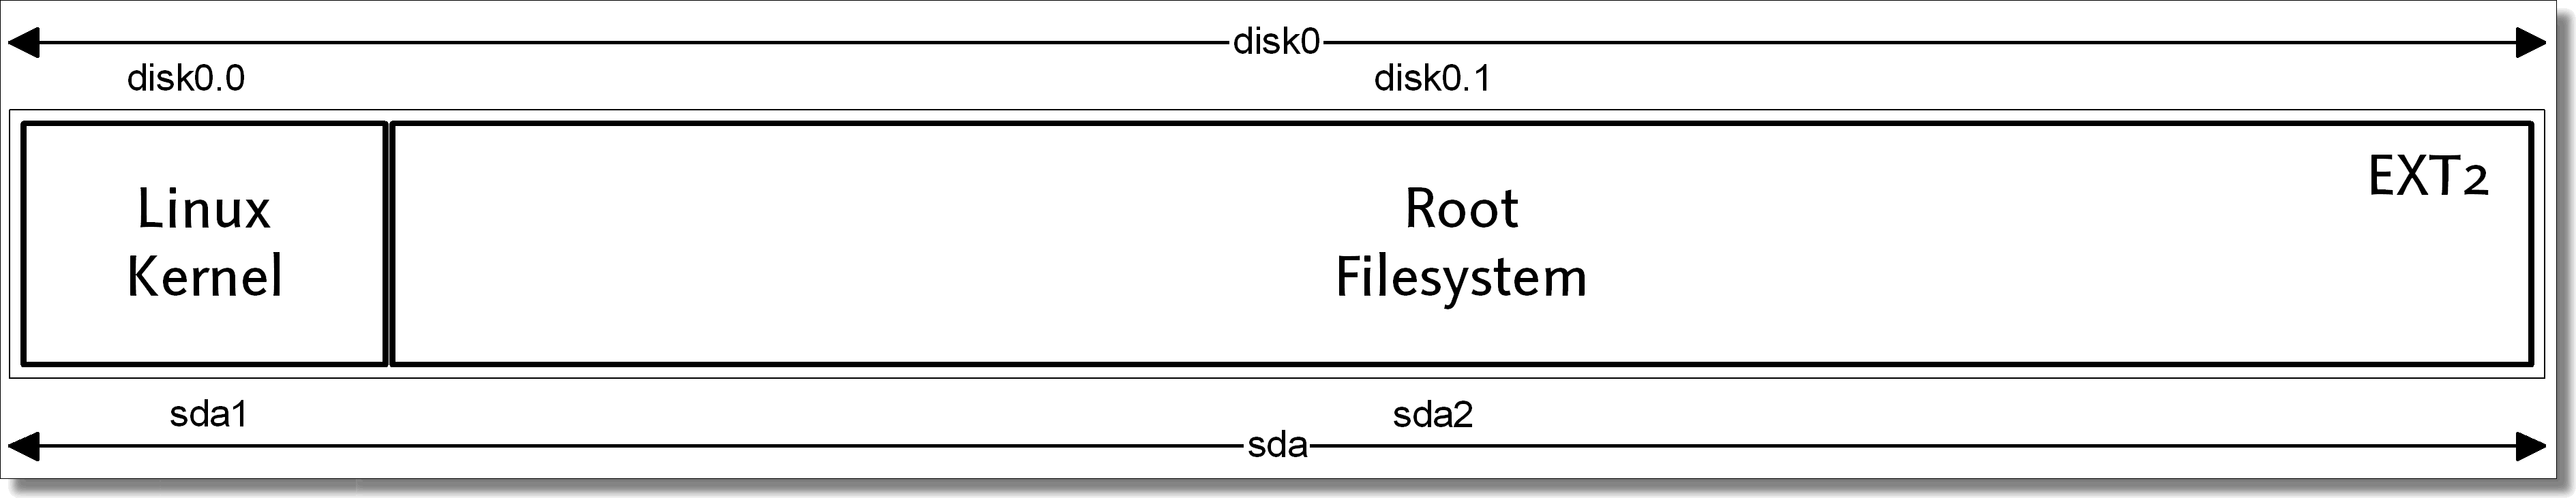
\includegraphics{OSELAS.BSP-Pengutronix-Mini2440/documentation/plain_sources/sd_card_partition.png}}

Note: The partition which contains the kernel image does not use any kind of
filesystem. So, the kernel's image is copied to the \textit{device}, not to
its \textit{filesystem}.

Persistent setup in the Barebox's \texttt{/env/config}.

\begin{ptxshell}[escapechar=|]{^}
kernel_loc=mmc
rootfs_loc=mmc
\end{ptxshell}

Specific settings in \texttt{/env/config} for the SD/MMC case:

\begin{ptxshell}[escapechar=|]{^}
rootfs_type=ext2
rootfs_mmc_part=2
kernel_mmc_part=0
kernelimage_type=uimage
\end{ptxshell}

With these settings Barebox will automatically load the kernel from the SD card
and instruct the kernel to also use the SD card as its root filesystem.
\texttt{kernel\_mmc\_part} defines the SD/MMC card's partition number to load the
kernel from. \texttt{rootfs\_mmc\_part} defines the partition on the SD/MMC card
the kernel should use as its root filesystem and \texttt{rootfs\_type}
defines the used filesystem. \texttt{kernelimage\_type} defines the type of the
kernel image, to make Barebox aware how to extract it.

Start manually:

\begin{ptxshell}[escapechar=|]{^}
mini2440:/ boot mmc
\end{ptxshell}

The manual start from the SD/MMC card requires the following specific settings
in the \texttt{/env/config}:

\begin{ptxshell}[escapechar=|]{^}
rootfs_type=ext2
rootfs_mmc_part=2
kernel_mmc_part=0
kernelimage_type=uimage
\end{ptxshell}

\section{Network Memory}				\label{sec:networkmem}

Using the network based method to boot the Mini2440 is more dedicated for
development. It simplifies replacing software in the kernel and root filesystem.
Also, the development cycle time can be reduced, with fewer opportunities for
making errors. All run-time relevant software parts are still
part of the development host in this case and can be easily changed on the
host and are instantly visible at the target's side.

To use the network based method this board support package creates the
following parts:

\begin{itemize}
\item \texttt{\ptxdistPlatformDir images/linuximage} is the Linux kernel
	and must be copied to the NFS or TFTP exported directory with a
	name the target expect it (in our case here for example
	\texttt{uImage-mini2440})
\item \texttt{\ptxdistPlatformDir root/} contains the root filesystem
	to be exported via NFS
\end{itemize}

\centerline{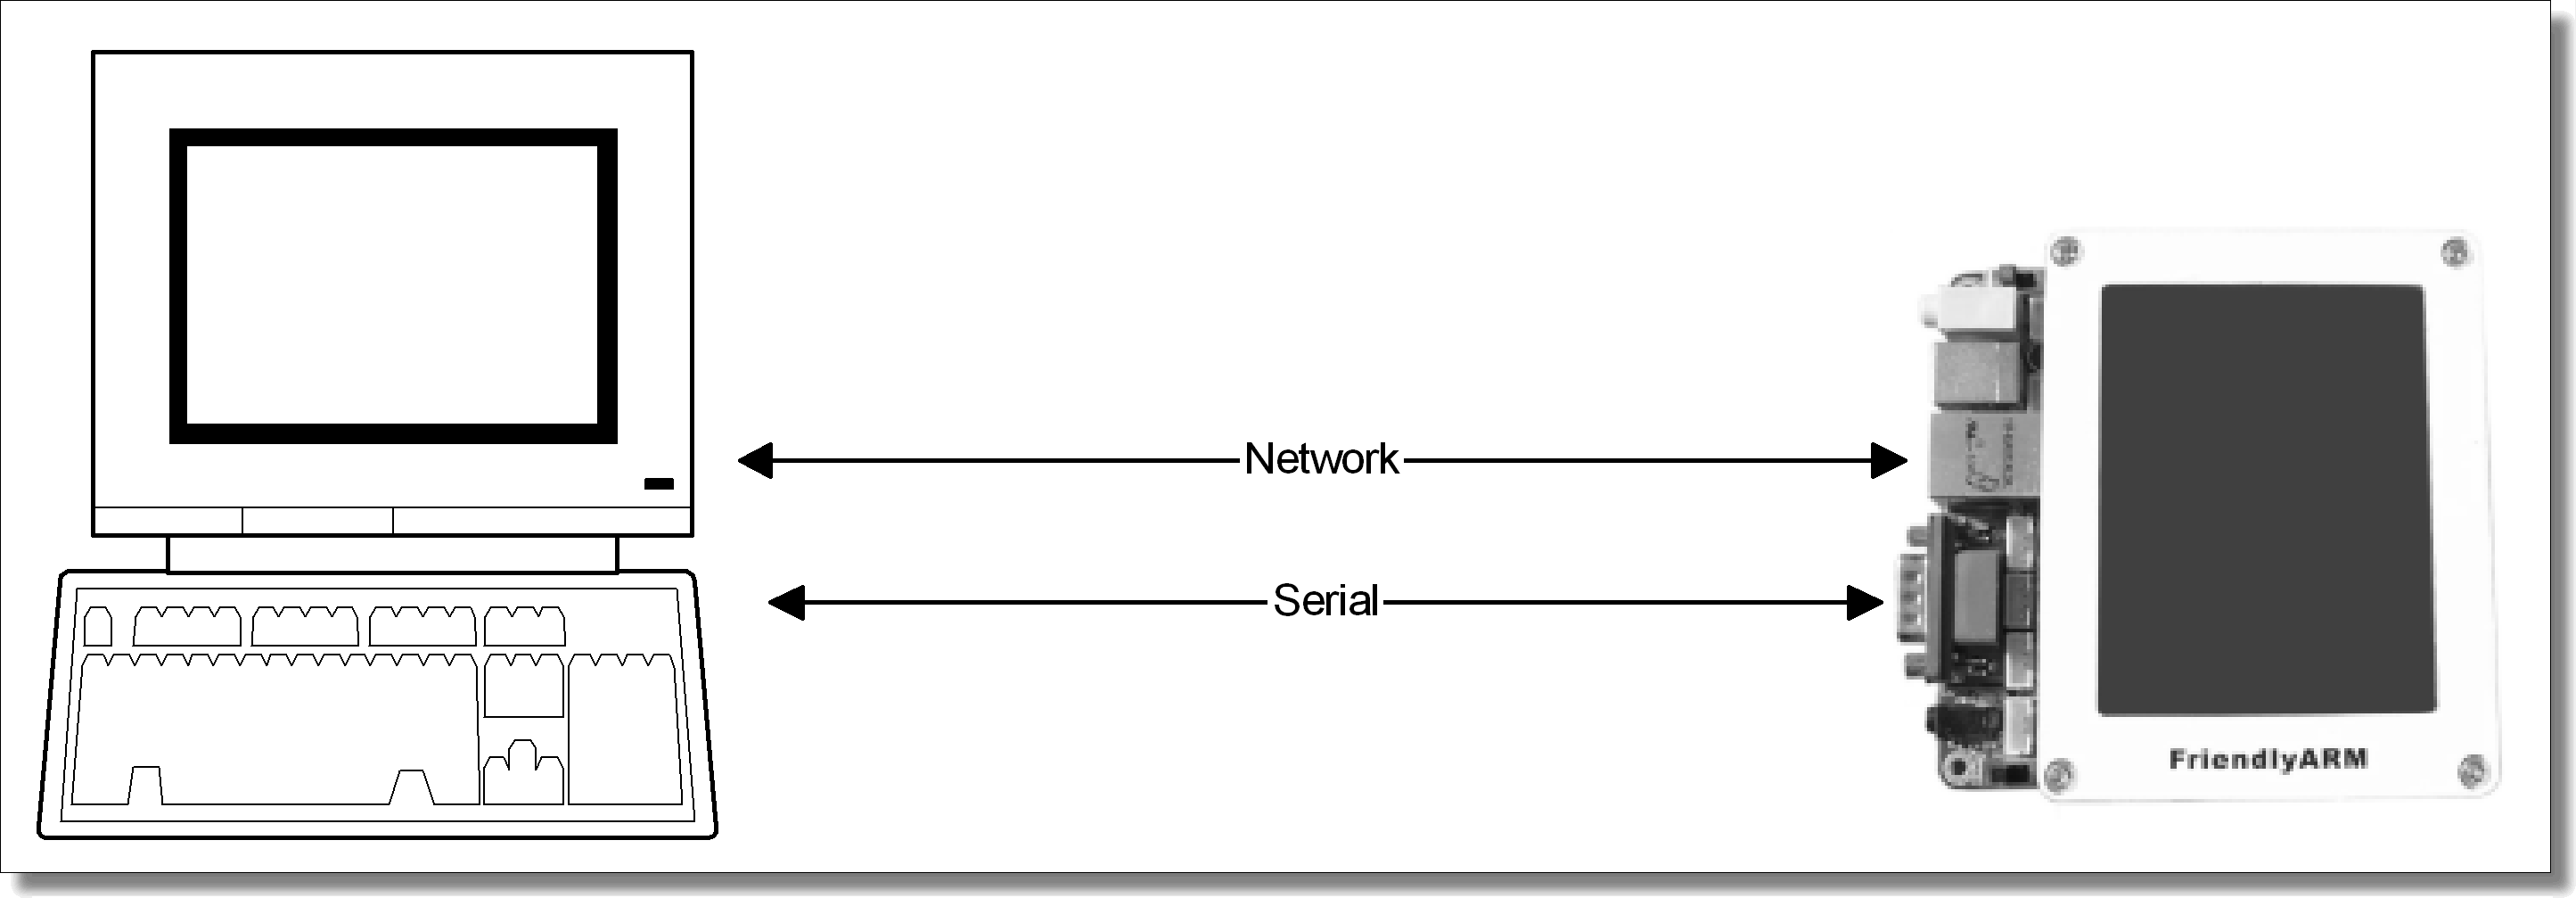
\includegraphics{OSELAS.BSP-Pengutronix-Mini2440/documentation/plain_sources/nfs_root.png}}

Persistent setup in the Barebox's \texttt{/env/config}.

Using the TFTP protocol for downloading the kernel:

\begin{ptxshell}[escapechar=|]{^}
kernel_loc=tftp
rootfs_loc=net
\end{ptxshell}

Specific settings in \texttt{/env/config} for the TFTP case:

\begin{ptxshell}[escapechar=|]{^}
kernelimage=uImage-mini2440
kernelimage_type=uimage
nfsroot="/path/to/nfs/root"
\end{ptxshell}

With these settings Barebox will automatically load the kernel with the name
\texttt{kernelimage} via network from a TFTP server and instruct it to use
the path given in \texttt{nfsroot} as its root filesystem.
\texttt{kernelimage\_type} defines the type of the kernel image, to make
Barebox aware how to extract it.

Using the NFS protocol for downloading the kernel:

\begin{ptxshell}[escapechar=|]{^}
kernel_loc=nfs
rootfs_loc=net
\end{ptxshell}

Specific settings in \texttt{/env/config} for the NFS case:

\begin{ptxshell}[escapechar=|]{^}
kernelimage=uImage-mini2440
kernelimage_type=uimage
nfsroot="/path/to/nfs/root"
\end{ptxshell}

With these settings Barebox will automatically load the kernel with the name
\texttt{kernelimage} via network from a NFS server and instruct it to use
the path given in \texttt{nfsroot} as its root filesystem.
\texttt{kernelimage\_type} defines the type of the kernel image, to make
Barebox aware how to extract it.

Start manually and download the kernel via TFTP:

\begin{ptxshell}[escapechar=|]{^}
mini2440:/ boot tftp
\end{ptxshell}

The manual start from a TFTP server requires the following specific settings
in the \texttt{/env/config}:

\begin{ptxshell}[escapechar=|]{^}
kernelimage=uImage-mini2440
kernelimage_type=uimage
nfsroot="/path/to/nfs/root"
\end{ptxshell}

Start manually and download the kernel via NFS:

\begin{ptxshell}[escapechar=|]{^}
mini2440:/ boot nfs
\end{ptxshell}

The manual start from an NFS server requires the following specific settings
in the \texttt{/env/config}:

\begin{ptxshell}[escapechar=|]{^}
kernelimage=uImage-mini2440
kernelimage_type=uimage
nfsroot="/path/to/nfs/root"
\end{ptxshell}

\section{Adaptions}

As mentioned above all settings are based on changes in a simple text file.
Whenever we run the 'boot' command, the script in \texttt{/env/bin/boot} is
called. So, adaptions can be made in \texttt{/env/config} to use one of the
supported boot methods in \texttt{/env/bin/boot}. For more complicated
scenarious also the \texttt{/env/bin/boot} can be changed. As it's a simple
shell script, it's very easy to adapt it to different requirements.
